\section{Evasión de Colisiones}
\setlength{\columnseprule}{0pt}
\onecolumn
\subsection{Polígono de Velocidades Admisibles}
Ramírez \& Zeghloul~\cite{ramirez2001control} modelan cada obstáculo como una restricción en el espacio de velocidades $(v,\omega)$ del robot, considerando la dirección del obstáculo respecto al robot.


\begin{figure}[H]
    \centering
    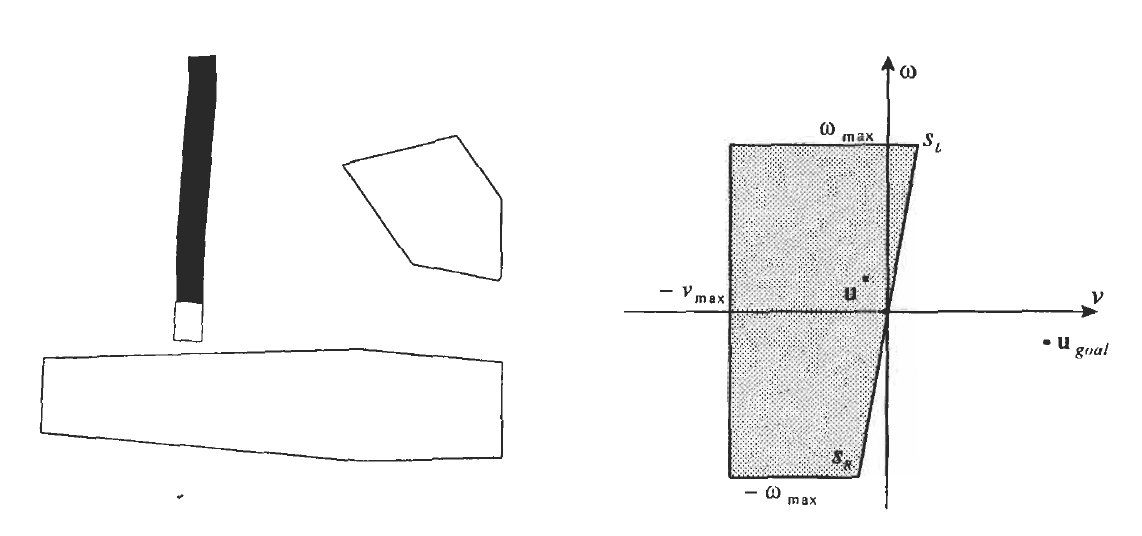
\includegraphics[width=0.6\linewidth]{pva.png}
    %\caption{La representación de obstáculos en el espacio de velocidades —de Ramírez y Zeghloul— fundamenta el PVA implementado en este proyecto}
    \label{fig:pva_antecedentes}
\end{figure}
